\documentclass[a4paper]{article}

\usepackage[T1]{fontenc}
\usepackage{titling}
\usepackage{amsmath}
\usepackage{amsfonts}
\usepackage{graphicx}
\usepackage{mathtools}
\usepackage[includeheadfoot,margin=1in]{geometry}

\usepackage{listings}

\usepackage{chngcntr}
\counterwithin{figure}{section}

\usepackage{caption}
\usepackage{subcaption}

\usepackage{fancyhdr}
\pagestyle{fancy}




\renewcommand{\headrulewidth}{0.5pt}

\numberwithin{equation}{section}
\usepackage[numbered, framed]{matlab-prettifier}

\lstset{
	style              = Matlab-editor,
	escapechar         = ",
	mlshowsectionrules = true,
	tabsize            = 2,
}



\setlength{\droptitle}{-8em}

\title{Homework 3 \\ \large Report}

\author{\textbf{A0153992U, A0000000U, A0000000U} \\ Team ChickenPox}

\date{}

\begin{document}

\maketitle

\section{Introduction}

\subsection{We are awesome}

Hello world!

\section{Feature generation}

Alike image recognition, natural language processing is something that our brains are accustomed to due to millions of years of evolution and fine tuning. We are very good at recognizing the important information and context contained in a written passage, but however natural it may seem, it is certainly not simple to imitate. Given a passage, how can we automatically extract the important information, and how do we connect this to formulate a coherent response?

In order to run machine learning classifiers on the given dataset we decided to play with a number of distinct methods for generating natural language features. Most are based on computing simple statistics such as the number of occurrences on the words or collections of words (bigrams). Some more sophisticated ones tried to also take into account the word order. All are described below.

\subsection{Bag of words}

The bag of words model is a simplistic representation of the natural language structure. Each word is treated as a seperate entity collected into an overall "bag" of words corresponding to the text being analysed. The bag can be then used to generate features (later fed into the classifier), which are commonly a simple statistic computed for a given word. One such statistic is occurence frequency, so simply the number of times a word appeared in a passage. This is expected to be expressive enough to reveal simple patterns, such as [if an object word (e.g. "apple") appears an even number of times, it is likely to be "picked up" and then "dropped"]. It is not, however, expressive enough to take into account even simple grammatical structure, supporting fact sequences and many others, that we, humans, spot immediately.
In our case the "bag of words" approach was easily implemented due to the favt that the test and validation sets were assumed to map to the same word dictionary. It should be noted, though, that if this is not the case, then either the dimension of the feature vector explodes to extremely large sizes, or we are pressed to detect the word type, such as "person" or "object", before we can proceed with the feature generation.

\subsection{N-grams}

Much more expressive structure of the text is revealed if "n-grams" are used instead of "1-grams", the single word features desribed above. N-grams are lists of subsequently occuring N words in the texts, such as "John picked up an apple" maps to a bag of 2-grams such as "[(John, picked), (picked, up), (up, an), (an, apple)]". The expressiveness arises because more intricate grammatical or logical patterns are contained when the words are combined. We can detect, for example, the relationship between the "person" and the "activity", as well as the "activity" and the "object", all of which contribute to much higher performance.

\subsection{Cantor mapping}

To achieve even higher expressiveness of the passage features, we decided to incorporate the absolute word order into the feature generation. The motivation behind it arises from the fact that the word order is, after all, what decides on the sense of a passage. If we know the interrelationship between the words' positions, we might be able to infer how each of them affects the final answer to the posed question.
The first iteration of the approach was an upgrade of the "bag of words" method described above. Instead of just counting the number of occurences, we computed the occurences' indices in the text, such as: \\

\noindent \textbf{"John picked up an apple. John dropped an apple"} \\
\textbf{bag of words}: featureValue("apple")=noOccurences("apple")=2 \\
\textbf{bag of words + word order}: featureValue("apple")=func(occurences("apple")=func([4,8])=? \\

Func is a function that maps the occurences of a word in a passage to a unique integer value. It is required because the datapoint for a particular feature and passage has to be a unique value, not an array.

The choice of func was a non-trivial task, as it had to be expressive enough for the classifier to figure out what the word order was from the unique integer value.

Disadvantages - Add sth like:
For uniqueMapping, it might not matter so much that the word is in the 15th or 25th position, as long as the noun is followed by a verb.

\section{Regularization and validation}

\section{Results}

\section{Improvements}

\begin{figure}[h!]
	\centering
	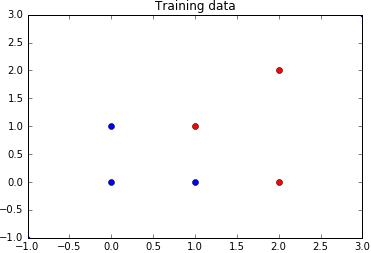
\includegraphics[page=1,width=0.60\textwidth]{diagram.png}
	\caption{\label{fig:diagram}{Hehehe}}
\end{figure}

\begin{lstlisting}[frame=single]
for i:=maxint to 0 do
begin
{ do nothing }
end;
Write('Case insensitive ');
Write('Pascal keywords.');
\end{lstlisting}

\end{document}